\titledquestion{Topological Sorting}

Consider the unweighted directed graph $G$ below. 

\begin{figure}[H]
    \centering
    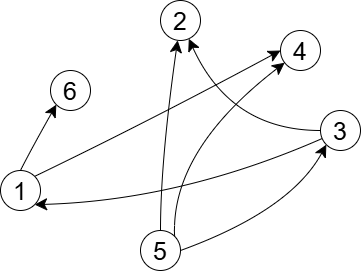
\includegraphics[width=0.5\linewidth]{fig/Topological_Sort.png}
    \label{fig:Topological_Sort}
\end{figure}

\begin{parts}

\part[5] 
How many topological sort results are there for the graph? State all possible results and show your calculated process.
\begin{solution}
    There are 8 topological sort results for the graph. They are as follows:
    \begin{center}
        5 3 1 2 4 6\\
        5 3 1 2 6 4\\
        5 3 1 4 2 6\\
        5 3 1 4 6 2\\
        5 3 1 6 2 4\\
        5 3 1 6 4 2\\
        5 3 2 1 4 6\\
        5 3 2 1 6 4
    \end{center}
    \textbf{Process:}
    \begin{enumerate}
        \item Find the vertices with zero in-degree.
        \item Remove the vertices with zero in-degree and their outgoing edges, then update the in-degree of the remaining vertices
        \item Repeat step 1 and 2 until all vertices are removed
    \end{enumerate}
    We can find that at first, only 5 has zero in-degree. So we can only remove 5 and its outgoing edges. Then we can find that only 3 has zero in-degree. So we can only remove 3 and its outgoing edges. This gives us the first two vertices in the topological sort: 5, 3\\
    Then, after removing 5 and 3, we can find that both 1 and 2 have zero in-degree. Now we have our first diverge. We first talk about the case where we choose 1 first. After removing 1 and its outgoing edges, we can find that all remaining vertices, 2 4 6, have zero in-degree. So we can remove them in any order. This gives us 6 types of topological sort: 5 3 1 2 4 6, 5 3 1 2 6 4, 5 3 1 4 2 6, 5 3 1 4 6 2, 5 3 1 6 2 4, 5 3 1 6 4 2.\\
    Then we talk about the case where we choose 2 first. After removing 2 and its outgoing edges, we can find that still only vertex 1 has zero in-degree. So we can remove 1 and its outgoing edges. After that both 4 and 6 have zero in-degree. So we can remove them in any order. This gives us 2 more types of topological sort: 5 3 2 1 4 6, 5 3 2 1 6 4.\\
    Thus we have 8 topological sort results for the graph.
\end{solution}
\vspace{5cm}


\part[5] 
Construct an example of a single directed edge that, when added to $G$, would make it impossible to create a valid topological ordering of the graph. Then, determine the total number of such edges that could be added to $G$ and explain why each of these edges prevents a topological ordering.\\
(Ensure that this edge is not a self-loop and does not duplicate an existing edge in $G$.)
\begin{solution}
    Example: add an edge from 6 to 5. This will make it impossible to create a valid topological ordering of the graph because at first step there is no vertex with zero in-degree.\\
    To find all the edges that could be added to $G$ to make it impossible to create a valid topological ordering, we can find all the edges such that it will make the graph has no vertex with zero in-degree at some point.\\
    For the first step, if we add an edge from an arbitrary vertex to 5, then there will be no vertex with zero in-degree. This will contribute to 5 edges that could be added to $G$ to make it impossible to create a valid topological ordering.\\
    Next, consider vertex 3. If we add an edge from an arbitrary vertex except 5 to 3, then there will be no vertex with zero in-degree after removing 5. This will contribute to 4 edges that could be added to $G$ to make it impossible to create a valid topological ordering.\\
    Next, we talk about the subgraph of 1 2 4 6. It is easy to see that in this subgraph, the only way to make it impossible to create a valid topological ordering is to add an edge that is a reverse of an existing edge(that is to say, add an edge from 4 to 1 or from 6 to 1). This will contribute to 2 edges that could be added to $G$ to make it impossible to create a valid topological ordering.\\
    Thus in total, there are 5+4+2=11 edges that could be added to $G$ to make it impossible to create a valid topological ordering.
\end{solution}

\vspace{5cm}

\end{parts}